\documentclass[a4paper]{article}
%
\usepackage{geometry}
\usepackage{tikz}
\usetikzlibrary{3d}
\usetikzlibrary{patterns}
\usepackage{ifthen}
\usetikzlibrary{backgrounds,fit}
\usetikzlibrary{calc}

\geometry{margin=2cm}

% Define colors
\definecolor{red}{RGB}{255,0,0}
\definecolor{green}{RGB}{0,255,0}
\definecolor{blue}{RGB}{0,0,255}
\definecolor{yellow}{RGB}{255,255,0}
\definecolor{white}{RGB}{255,255,255}
\definecolor{orange}{RGB}{255,165,0}

% Define the function to draw a single cubicle
\newcommand{\drawcubicle}[5][X]{
  \ifthenelse{\equal{#1}{X}}{
  \begin{scope}[shift={#2}]
    % Front face
    \begin{scope}[canvas is xy plane at z=0]
      \path[draw=black,#3] (0,0) rectangle (1,1);
    \end{scope}
    % Top face
    \begin{scope}[canvas is xz plane at y=1]
      \path[draw=black,#4] (0,0) rectangle (1,1);
    \end{scope}
    % Right face
    \begin{scope}[canvas is yz plane at x=1]
      \path[draw=black,#5] (0,0) rectangle (1,1);
    \end{scope}
  \end{scope}
}{}
}

\newcommand{\cubeCanvas}{
  % Draw the Rubik's Cube
  \foreach \x in {0,1,2} {
    \foreach \y in {0,1,2} {
      \foreach \z in {2,1,0} {
        \drawcubicle{(\x,\y,\z)}{draw=white}{draw=white}{draw=white}
      }
    }
  }
}


\pgfdeclarepatternformonly{upwards arrows}
  {\pgfpointorigin}{\pgfpoint{1cm}{0.3cm}}{\pgfpoint{1cm}{0.3cm}}
  {
  % Draw the triangles
  \pgfpathmoveto{\pgfpoint{0}{0}}
  \pgfpathlineto{\pgfpoint{0.25cm}{0}}
  \pgfpathlineto{\pgfpoint{0.5cm}{0.15cm}}
  \pgfpathlineto{\pgfpoint{0.75cm}{0}}
  \pgfpathlineto{\pgfpoint{1cm}{0}}
  \pgfpathlineto{\pgfpoint{0.5cm}{0.3cm}}
  \pgfpathlineto{\pgfpoint{0}{0}}
  \pgfpathclose
  \pgfusepath{fill}
}

\tikzset{inner/.style={fill=gray!50!white,draw=black}}



\title{Alain's Rubik's Methods}
\author{Alain Lehmann}

\begin{document}

\maketitle
%\tableofcontents

\raggedright
\section{Mnemonics}
\centering

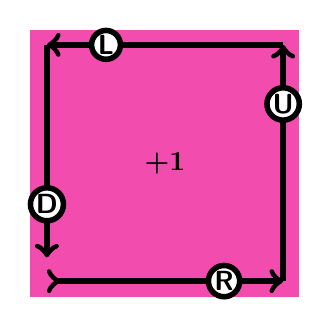
\begin{tikzpicture}
\tikzset{arrowlabel/.style={pos=0.75,draw=black,fill=white,circle,inner sep=0.5pt,font=\sffamily\bfseries}}
\tikzset{ultrathick/.style={line width=2}}
\begin{scope}[local bounding box=BB,scale=1.5]
  \draw (0,0) coordinate(X);
  \draw[>->,ultrathick] (X) -- ++(2,0) node[arrowlabel]{R} coordinate(X);
  \draw[->,ultrathick] (X) -- ++(0,2) node[arrowlabel]{U} coordinate(X);
  \draw[->,ultrathick] (X) -- ++(-2,0) node[arrowlabel]{L} coordinate(X);
  \draw[->,ultrathick] (X) -- ++(0,-1.8) node[arrowlabel]{D} coordinate(X);
  \draw (1,1) node{\bf +1};
  \begin{pgfonlayer}{background}
    \fill[magenta,opacity=0.7] (BB.north west) rectangle (BB.south east);
  \end{pgfonlayer}
\end{scope}
\end{tikzpicture}%
%
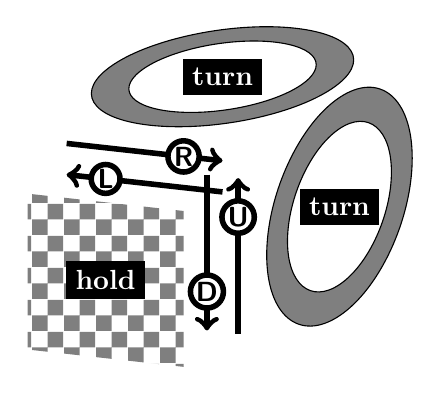
\begin{tikzpicture}
\tikzset{top/.style={fill=green}}
\tikzset{bottom/.style={fill=blue}}
\tikzset{right/.style={fill=red}}
\tikzset{left/.style={fill=orange}}
\tikzset{front/.style={fill=yellow}}
\tikzset{back/.style={fill=white}}
\tikzset{ultrathick/.style={line width=2}}
\tikzset{arrowlabel/.style={pos=0.75,draw=black,fill=white,circle,inner sep=0.5pt,font=\sffamily\bfseries}}
\begin{scope}
  [x={(0.9cm,-0.1cm)},y={(0,0.9cm)},z={(0.6cm,0.4cm)},scale=1.1]
% BACK
\drawCubicleNorthEast[X]{-1}{-1}{2}
\drawCubicleNorthEast[X]{-1}{-0}{2}
\drawCubicleNorthEast[X]{-0}{-1}{2}
\drawCubicleNorthEast[X]{-1}{+1}{2}
\drawCubicleNorthEast[X]{-0}{+0}{2}
\drawCubicleNorthEast[X]{+1}{-1}{2}
\drawCubicleNorthEast[X]{-0}{+1}{2}
\drawCubicleNorthEast[X]{+1}{-0}{2}
\drawCubicleNorthEast[X]{+1}{+1}{2}
%MIDDLE
\drawCubicleNorthEast[X]{-1}{-1}{1}
\drawCubicleNorthEast[X]{-1}{-0}{1}
\drawCubicleNorthEast[X]{-0}{-1}{1}
\drawCubicleNorthEast[X]{-1}{+1}{1}
\drawCubicleNorthEast[X]{-0}{+0}{1}
\drawCubicleNorthEast[X]{+1}{-1}{1}
\drawCubicleNorthEast[X]{-0}{+1}{1}
\drawCubicleNorthEast[X]{+1}{-0}{1}
\drawCubicleNorthEast[X]{+1}{+1}{1}
% FRONT
\drawCubicleNorthEast[X]{-1}{-1}{0}
\drawCubicleNorthEast[X]{-1}{-0}{0}
\drawCubicleNorthEast[X]{-0}{-1}{0}
\drawCubicleNorthEast[X]{-1}{+1}{0}
\drawCubicleNorthEast[X]{-0}{+0}{0}
\drawCubicleNorthEast[X]{+1}{-1}{0}
\drawCubicleNorthEast[X]{-0}{+1}{0}
\drawCubicleNorthEast[X]{+1}{-0}{0}
\drawCubicleNorthEast[X]{+1}{+1}{0}
%% FRONT
  \begin{scope}[canvas is xz plane at y=2.0]
    \draw[fill=black, fill opacity=0.5,even odd rule]
      (0.5,1.5) circle (1.4)
      (0.5,1.5) circle (1.0)
    ;
    \draw (0.5,1.5) node[text=white,fill=black] {\bf turn};
  \end{scope}
  \begin{scope}[canvas is yz plane at x=2.0]
    \draw[fill=black, fill opacity=0.5,even odd rule]
      (0.5,1.5) circle (1.4)
      (0.5,1.5) circle (1.0)
    ;
    \draw (0.5,1.5) node[text=white,fill=black] {\bf turn};
  \end{scope}
  \begin{scope}[canvas is xy plane at z=0]
    \fill[pattern=checkerboard,opacity=0.5] (-1,-1) rectangle ++(2,2) node[midway,opacity=1,text=white,fill=black]{\bf hold};
    \draw[->,ultrathick] (-0.5,+1.5+0.2) -- ++(2.0,0) node[arrowlabel]{R};
    \draw[->,ultrathick] (+1.5+0.2,-0.5) -- ++(0,2.0) node[arrowlabel]{U};
    \draw[->,ultrathick] (-0.5+2,+1.5-0.2) -- ++(-2.0,0) node[arrowlabel]{L};
    \draw[->,ultrathick] (+1.5-0.2,-0.5+2) -- ++(0,-2.0) node[arrowlabel]{D};
  \end{scope}
\end{scope}

\end{tikzpicture}%
%
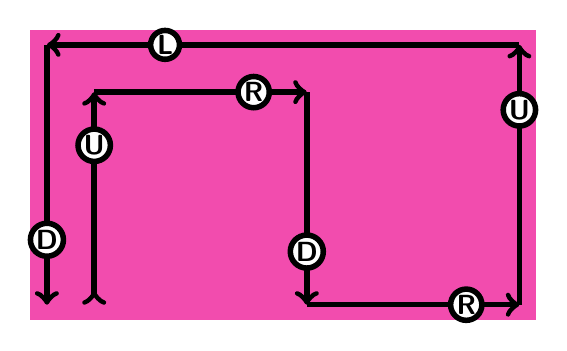
\begin{tikzpicture}
  \tikzset{ultrathick/.style={line width=2}}
  \tikzset{arrowlabel/.style={pos=0.75,draw=black,fill=white,circle,inner sep=0.5pt,font=\sffamily\bfseries}}
  \tikzset{rotarrow/.style={->, shorten >=4, shorten <=4, line width=2}}
  \tikzset{movarrow/.style={->, line width=2}}

  \begin{scope}[scale=3.0,local bounding box=BB]
  \path (0.1,0) coordinate (x);
    \draw[movarrow,>->] (x) -- ++(0,+0.9) coordinate(x) node[arrowlabel]{U};
    \draw[movarrow] (x) -- ++(+0.9,+0) coordinate(x) node[arrowlabel]{R};
    \draw[movarrow] (x) -- ++(0,-0.9) coordinate(x) node[arrowlabel]{D};
    \draw[movarrow] (x) -- ++(+0.9,0) coordinate(x) node[arrowlabel]{R};
    \draw[movarrow] (x) -- ++(0,+1.1) coordinate(x) node[arrowlabel]{U};
    \draw[movarrow] (x) -- ++(-2,0) coordinate(x) node[arrowlabel]{L};
    \draw[movarrow] (x) -- ++(0,-1.1) coordinate(x) node[arrowlabel]{D};
    \begin{pgfonlayer}{background}
      \fill[magenta,opacity=0.7] (BB.north west) rectangle (BB.south east);
    \end{pgfonlayer}
  \end{scope}
\end{tikzpicture}

\raggedright
\section{Solution process}
\centering

\tikzset{front/.style={fill=red}}
\tikzset{top/.style={fill=white}}
\tikzset{right/.style={fill=blue}}
\begin{tikzpicture}[z={(0.5cm,0.5cm)}]
  \cubeCanvas
%%%% BOTTOM
\drawcubicle[_]{(0,0,2)}{inner}{inner}{inner} % 1
\drawcubicle[_]{(1,0,2)}{inner}{inner}{inner} %   2
\drawcubicle[_]{(2,0,2)}{inner}{inner}{right} %     3
\drawcubicle[_]{(0,0,1)}{inner}{inner}{inner} % 4
\drawcubicle[X]{(1,0,1)}{inner}{inner}{inner} %   5
\drawcubicle[_]{(2,0,1)}{inner}{inner}{right} %     6
\drawcubicle[_]{(0,0,0)}{front}{inner}{inner} % 7
\drawcubicle[_]{(1,0,0)}{front}{inner}{inner} %   8
\drawcubicle[_]{(2,0,0)}{front}{inner}{right} %     9
%%
%%%% MIDDLE
\drawcubicle[_]{(0,1,2)}{inner}{inner}{inner} % 1
\drawcubicle[X]{(1,1,2)}{inner}{inner}{inner} %   2
\drawcubicle[_]{(2,1,2)}{inner}{inner}{right} %     3
\drawcubicle[X]{(0,1,1)}{inner}{inner}{inner} % 4
\drawcubicle[X]{(1,1,1)}{inner}{inner}{inner} %   5
\drawcubicle[X]{(2,1,1)}{inner}{inner}{right} %     6
\drawcubicle[_]{(0,1,0)}{front}{inner}{inner} % 7
\drawcubicle[X]{(1,1,0)}{front}{inner}{inner} %   8
\drawcubicle[_]{(2,1,0)}{front}{inner}{right} %     9
%%
%%%% TOP
\drawcubicle[_]{(0,2,2)}{inner}{top}{inner} % 1
\drawcubicle[_]{(1,2,2)}{inner}{top}{inner} %   2
\drawcubicle[_]{(2,2,2)}{inner}{top}{right} %     3
\drawcubicle[_]{(0,2,1)}{inner}{top}{inner} % 4
\drawcubicle[X]{(1,2,1)}{inner}{top}{inner} %   5
\drawcubicle[_]{(2,2,1)}{inner}{top}{right} %     6
\drawcubicle[_]{(0,2,0)}{front}{top}{inner} % 7
\drawcubicle[_]{(1,2,0)}{front}{top}{inner} %   8
\drawcubicle[_]{(2,2,0)}{front}{top}{right} %     9
%%
\end{tikzpicture}%
%
\begin{tikzpicture}
  [x={(0.9cm,-0.1cm)},y={(0,0.9cm)},z={(0.6cm,0.4cm)}]
  \cubeCanvas
%%%% BOTTOM
\drawcubicle[_]{(0,0,2)}{inner}{inner}{inner} % 1
\drawcubicle[_]{(1,0,2)}{inner}{inner}{inner} %   2
\drawcubicle[_]{(2,0,2)}{inner}{inner}{right} %     3
\drawcubicle[_]{(0,0,1)}{inner}{inner}{inner} % 4
\drawcubicle[X]{(1,0,1)}{inner}{inner}{inner} %   5
\drawcubicle[_]{(2,0,1)}{inner}{inner}{right} %     6
\drawcubicle[_]{(0,0,0)}{front}{inner}{inner} % 7
\drawcubicle[_]{(1,0,0)}{front}{inner}{inner} %   8
\drawcubicle[_]{(2,0,0)}{front}{inner}{right} %     9
%%
%%%% MIDDLE
\drawcubicle[_]{(0,1,2)}{inner}{inner}{inner} % 1
\drawcubicle[X]{(1,1,2)}{inner}{inner}{inner} %   2
\drawcubicle[_]{(2,1,2)}{inner}{inner}{right} %     3
\drawcubicle[X]{(0,1,1)}{inner}{inner}{inner} % 4
\drawcubicle[X]{(1,1,1)}{inner}{inner}{inner} %   5
\drawcubicle[X]{(2,1,1)}{inner}{inner}{right} %     6
\drawcubicle[_]{(0,1,0)}{front}{inner}{inner} % 7
\drawcubicle[X]{(1,1,0)}{front}{inner}{inner} %   8
\drawcubicle[_]{(2,1,0)}{front}{inner}{right} %     9
%%
%%%% TOP
\drawcubicle[_]{(0,2,2)}{inner}{top}{inner} % 1
\drawcubicle[X]{(1,2,2)}{inner}{top}{inner} %   2
\drawcubicle[_]{(2,2,2)}{inner}{top}{right} %     3
\drawcubicle[X]{(0,2,1)}{inner}{top}{inner} % 4
\drawcubicle[X]{(1,2,1)}{inner}{top}{inner} %   5
\drawcubicle[X]{(2,2,1)}{inner}{top}{right} %     6
\drawcubicle[_]{(0,2,0)}{front}{top}{inner} % 7
\drawcubicle[X]{(1,2,0)}{front}{top}{inner} %   8
\drawcubicle[_]{(2,2,0)}{front}{top}{right} %     9
%%
\end{tikzpicture}%
%
\begin{tikzpicture}
  [x={(0.9cm,-0.1cm)},y={(0,0.9cm)},z={(0.6cm,0.4cm)}]
  \cubeCanvas
%%%% BOTTOM
\drawcubicle[_]{(0,0,2)}{inner}{inner}{inner} % 1
\drawcubicle[_]{(1,0,2)}{inner}{inner}{inner} %   2
\drawcubicle[_]{(2,0,2)}{inner}{inner}{right} %     3
\drawcubicle[_]{(0,0,1)}{inner}{inner}{inner} % 4
\drawcubicle[X]{(1,0,1)}{inner}{inner}{inner} %   5
\drawcubicle[_]{(2,0,1)}{inner}{inner}{right} %     6
\drawcubicle[_]{(0,0,0)}{front}{inner}{inner} % 7
\drawcubicle[_]{(1,0,0)}{front}{inner}{inner} %   8
\drawcubicle[_]{(2,0,0)}{front}{inner}{right} %     9
%%
%%%% MIDDLE
\drawcubicle[_]{(0,1,2)}{inner}{inner}{inner} % 1
\drawcubicle[X]{(1,1,2)}{inner}{inner}{inner} %   2
\drawcubicle[_]{(2,1,2)}{inner}{inner}{right} %     3
\drawcubicle[X]{(0,1,1)}{inner}{inner}{inner} % 4
\drawcubicle[X]{(1,1,1)}{inner}{inner}{inner} %   5
\drawcubicle[X]{(2,1,1)}{inner}{inner}{right} %     6
\drawcubicle[_]{(0,1,0)}{front}{inner}{inner} % 7
\drawcubicle[X]{(1,1,0)}{front}{inner}{inner} %   8
\drawcubicle[_]{(2,1,0)}{front}{inner}{right} %     9
%%
%%%% TOP
\drawcubicle[X]{(0,2,2)}{inner}{top}{inner} % 1
\drawcubicle[X]{(1,2,2)}{inner}{top}{inner} %   2
\drawcubicle[X]{(2,2,2)}{inner}{top}{right} %     3
\drawcubicle[X]{(0,2,1)}{inner}{top}{inner} % 4
\drawcubicle[X]{(1,2,1)}{inner}{top}{inner} %   5
\drawcubicle[X]{(2,2,1)}{inner}{top}{right} %     6
\drawcubicle[X]{(0,2,0)}{front}{top}{inner} % 7
\drawcubicle[X]{(1,2,0)}{front}{top}{inner} %   8
\drawcubicle[_]{(2,2,0)}{front}{top}{right} %     9
%%
\end{tikzpicture}%
%

\tikzset{front/.style={fill=blue}}
\tikzset{top/.style={fill=yellow}}
\tikzset{right/.style={fill=red}}
\begin{tikzpicture}[z={(0.5cm,0.5cm)}]
  \cubeCanvas
%%%% BOTTOM
\drawcubicle[X]{(0,0,2)}{inner}{inner}{inner} % 1
\drawcubicle[X]{(1,0,2)}{inner}{inner}{inner} %   2
\drawcubicle[X]{(2,0,2)}{inner}{inner}{right} %     3
\drawcubicle[X]{(0,0,1)}{inner}{inner}{inner} % 4
\drawcubicle[X]{(1,0,1)}{inner}{inner}{inner} %   5
\drawcubicle[X]{(2,0,1)}{inner}{inner}{right} %     6
\drawcubicle[X]{(0,0,0)}{front}{inner}{inner} % 7
\drawcubicle[X]{(1,0,0)}{front}{inner}{inner} %   8
\drawcubicle[_]{(2,0,0)}{front}{inner}{right} %     9
%%
%%%% MIDDLE
\drawcubicle[_]{(0,1,2)}{inner}{inner}{inner} % 1
\drawcubicle[X]{(1,1,2)}{inner}{inner}{inner} %   2
\drawcubicle[_]{(2,1,2)}{inner}{inner}{right} %     3
\drawcubicle[X]{(0,1,1)}{inner}{inner}{inner} % 4
\drawcubicle[X]{(1,1,1)}{inner}{inner}{inner} %   5
\drawcubicle[X]{(2,1,1)}{inner}{inner}{right} %     6
\drawcubicle[_]{(0,1,0)}{front}{inner}{inner} % 7
\drawcubicle[X]{(1,1,0)}{front}{inner}{inner} %   8
\drawcubicle[_]{(2,1,0)}{front}{inner}{right} %     9
%%
%%%% TOP
\drawcubicle[_]{(0,2,2)}{inner}{top}{inner} % 1
\drawcubicle[_]{(1,2,2)}{inner}{top}{inner} %   2
\drawcubicle[_]{(2,2,2)}{inner}{top}{right} %     3
\drawcubicle[_]{(0,2,1)}{inner}{top}{inner} % 4
\drawcubicle[X]{(1,2,1)}{inner}{top}{inner} %   5
\drawcubicle[_]{(2,2,1)}{inner}{top}{right} %     6
\drawcubicle[_]{(0,2,0)}{front}{top}{inner} % 7
\drawcubicle[_]{(1,2,0)}{front}{top}{inner} %   8
\drawcubicle[_]{(2,2,0)}{front}{top}{right} %     9
%%
\end{tikzpicture}%
%
\begin{tikzpicture}
  [x={(0.9cm,-0.1cm)},y={(0,0.9cm)},z={(0.6cm,0.4cm)}]
  \cubeCanvas
%%%% BOTTOM
\drawcubicle[X]{(0,0,2)}{inner}{inner}{inner} % 1
\drawcubicle[X]{(1,0,2)}{inner}{inner}{inner} %   2
\drawcubicle[X]{(2,0,2)}{inner}{inner}{right} %     3
\drawcubicle[X]{(0,0,1)}{inner}{inner}{inner} % 4
\drawcubicle[X]{(1,0,1)}{inner}{inner}{inner} %   5
\drawcubicle[X]{(2,0,1)}{inner}{inner}{right} %     6
\drawcubicle[X]{(0,0,0)}{front}{inner}{inner} % 7
\drawcubicle[X]{(1,0,0)}{front}{inner}{inner} %   8
\drawcubicle[_]{(2,0,0)}{front}{inner}{right} %     9
%%
%%%% MIDDLE
\drawcubicle[X]{(0,1,2)}{inner}{inner}{inner} % 1
\drawcubicle[X]{(1,1,2)}{inner}{inner}{inner} %   2
\drawcubicle[X]{(2,1,2)}{inner}{inner}{right} %     3
\drawcubicle[X]{(0,1,1)}{inner}{inner}{inner} % 4
\drawcubicle[X]{(1,1,1)}{inner}{inner}{inner} %   5
\drawcubicle[X]{(2,1,1)}{inner}{inner}{right} %     6
\drawcubicle[X]{(0,1,0)}{front}{inner}{inner} % 7
\drawcubicle[X]{(1,1,0)}{front}{inner}{inner} %   8
\drawcubicle[_]{(2,1,0)}{front}{inner}{right} %     9
%%
%%%% TOP
\drawcubicle[_]{(0,2,2)}{inner}{top}{inner} % 1
\drawcubicle[_]{(1,2,2)}{inner}{top}{inner} %   2
\drawcubicle[_]{(2,2,2)}{inner}{top}{right} %     3
\drawcubicle[_]{(0,2,1)}{inner}{top}{inner} % 4
\drawcubicle[X]{(1,2,1)}{inner}{top}{inner} %   5
\drawcubicle[_]{(2,2,1)}{inner}{top}{right} %     6
\drawcubicle[_]{(0,2,0)}{front}{top}{inner} % 7
\drawcubicle[_]{(1,2,0)}{front}{top}{inner} %   8
\drawcubicle[_]{(2,2,0)}{front}{top}{right} %     9
%%
\end{tikzpicture}%
%
\begin{tikzpicture}
  [x={(0.9cm,-0.1cm)},y={(0,0.9cm)},z={(0.6cm,0.4cm)}]
  \cubeCanvas
%%%% BOTTOM
\drawcubicle[X]{(0,0,2)}{inner}{inner}{inner} % 1
\drawcubicle[X]{(1,0,2)}{inner}{inner}{inner} %   2
\drawcubicle[X]{(2,0,2)}{inner}{inner}{right} %     3
\drawcubicle[X]{(0,0,1)}{inner}{inner}{inner} % 4
\drawcubicle[X]{(1,0,1)}{inner}{inner}{inner} %   5
\drawcubicle[X]{(2,0,1)}{inner}{inner}{right} %     6
\drawcubicle[X]{(0,0,0)}{front}{inner}{inner} % 7
\drawcubicle[X]{(1,0,0)}{front}{inner}{inner} %   8
\drawcubicle[_]{(2,0,0)}{front}{inner}{right} %     9
%%
%%%% MIDDLE
\drawcubicle[X]{(0,1,2)}{inner}{inner}{inner} % 1
\drawcubicle[X]{(1,1,2)}{inner}{inner}{inner} %   2
\drawcubicle[X]{(2,1,2)}{inner}{inner}{right} %     3
\drawcubicle[X]{(0,1,1)}{inner}{inner}{inner} % 4
\drawcubicle[X]{(1,1,1)}{inner}{inner}{inner} %   5
\drawcubicle[X]{(2,1,1)}{inner}{inner}{right} %     6
\drawcubicle[X]{(0,1,0)}{front}{inner}{inner} % 7
\drawcubicle[X]{(1,1,0)}{front}{inner}{inner} %   8
\drawcubicle[X]{(2,1,0)}{front}{inner}{right} %     9
%%
%%%% TOP
\drawcubicle[_]{(0,2,2)}{inner}{top}{inner} % 1
\drawcubicle[X]{(1,2,2)}{inner}{top}{inner} %   2
\drawcubicle[_]{(2,2,2)}{inner}{top}{right} %     3
\drawcubicle[X]{(0,2,1)}{inner}{top}{inner} % 4
\drawcubicle[X]{(1,2,1)}{inner}{top}{inner} %   5
\drawcubicle[X]{(2,2,1)}{inner}{top}{right,pattern=checkerboard} %     6
\drawcubicle[_]{(0,2,0)}{front}{top}{inner} % 7
\drawcubicle[X]{(1,2,0)}{front,pattern=checkerboard}{top}{inner} %   8
\drawcubicle[_]{(2,2,0)}{front}{top}{right} %     9
%%
\end{tikzpicture}%
%

\begin{tikzpicture}[z={(0.5cm,0.5cm)}]
  \cubeCanvas
%%%% BOTTOM
\drawcubicle[X]{(0,0,2)}{inner}{inner}{inner} % 1
\drawcubicle[X]{(1,0,2)}{inner}{inner}{inner} %   2
\drawcubicle[X]{(2,0,2)}{inner}{inner}{right} %     3
\drawcubicle[X]{(0,0,1)}{inner}{inner}{inner} % 4
\drawcubicle[X]{(1,0,1)}{inner}{inner}{inner} %   5
\drawcubicle[X]{(2,0,1)}{inner}{inner}{right} %     6
\drawcubicle[X]{(0,0,0)}{front}{inner}{inner} % 7
\drawcubicle[X]{(1,0,0)}{front}{inner}{inner} %   8
\drawcubicle[_]{(2,0,0)}{front}{inner}{right} %     9
%%
%%%% MIDDLE
\drawcubicle[X]{(0,1,2)}{inner}{inner}{inner} % 1
\drawcubicle[X]{(1,1,2)}{inner}{inner}{inner} %   2
\drawcubicle[X]{(2,1,2)}{inner}{inner}{right} %     3
\drawcubicle[X]{(0,1,1)}{inner}{inner}{inner} % 4
\drawcubicle[X]{(1,1,1)}{inner}{inner}{inner} %   5
\drawcubicle[X]{(2,1,1)}{inner}{inner}{right} %     6
\drawcubicle[X]{(0,1,0)}{front}{inner}{inner} % 7
\drawcubicle[X]{(1,1,0)}{front}{inner}{inner} %   8
\drawcubicle[X]{(2,1,0)}{front}{inner}{right} %     9
%%
%%%% TOP
\drawcubicle[_]{(0,2,2)}{inner}{top}{inner} % 1
\drawcubicle[X]{(1,2,2)}{inner}{top}{inner} %   2
\drawcubicle[_]{(2,2,2)}{inner}{top}{right} %     3
\drawcubicle[X]{(0,2,1)}{inner}{top}{inner} % 4
\drawcubicle[X]{(1,2,1)}{inner}{top}{inner} %   5
\drawcubicle[X]{(2,2,1)}{inner}{top}{right} %     6
\drawcubicle[_]{(0,2,0)}{front}{top}{inner} % 7
\drawcubicle[X]{(1,2,0)}{front}{top}{inner} %   8
\drawcubicle[_]{(2,2,0)}{front}{top}{right} %     9
%%
\end{tikzpicture}
%
\tikzset{front/.style={fill=red}}
\tikzset{top/.style={fill=green}}
\tikzset{right/.style={fill=white}}
\begin{tikzpicture}[z={(0.5cm,0.5cm)}]
  \cubeCanvas
%%%% BOTTOM
\drawcubicle[_]{(0,0,2)}{inner}{inner}{inner} % 1
\drawcubicle[X]{(1,0,2)}{inner}{inner}{inner} %   2
\drawcubicle[X]{(2,0,2)}{inner}{inner}{right} %     3
\drawcubicle[X]{(0,0,1)}{inner}{inner}{inner} % 4
\drawcubicle[X]{(1,0,1)}{inner}{inner}{inner} %   5
\drawcubicle[X]{(2,0,1)}{inner}{inner}{right} %     6
\drawcubicle[_]{(0,0,0)}{front}{inner}{inner} % 7
\drawcubicle[X]{(1,0,0)}{front}{inner}{inner} %   8
\drawcubicle[_]{(2,0,0)}{front}{inner}{right} %     9
%%
%%%% MIDDLE
\drawcubicle[X]{(0,1,2)}{inner}{inner}{inner} % 1
\drawcubicle[X]{(1,1,2)}{inner}{inner}{inner} %   2
\drawcubicle[X]{(2,1,2)}{inner}{inner}{right} %     3
\drawcubicle[X]{(0,1,1)}{inner}{inner}{inner} % 4
\drawcubicle[X]{(1,1,1)}{inner}{inner}{inner} %   5
\drawcubicle[X]{(2,1,1)}{inner}{inner}{right} %     6
\drawcubicle[X]{(0,1,0)}{front}{inner}{inner} % 7
\drawcubicle[X]{(1,1,0)}{front}{inner}{inner} %   8
\drawcubicle[X]{(2,1,0)}{front}{inner}{right} %     9
%%
%%%% TOP
\drawcubicle[_]{(0,2,2)}{inner}{top}{inner} % 1
\drawcubicle[X]{(1,2,2)}{inner}{top}{inner} %   2
\drawcubicle[X]{(2,2,2)}{inner}{top}{right} %     3
\drawcubicle[X]{(0,2,1)}{inner}{top}{inner} % 4
\drawcubicle[X]{(1,2,1)}{inner}{top}{inner} %   5
\drawcubicle[X]{(2,2,1)}{inner}{top}{right} %     6
\drawcubicle[_]{(0,2,0)}{front}{top}{inner} % 7
\drawcubicle[X]{(1,2,0)}{front}{top}{inner} %   8
\drawcubicle[X]{(2,2,0)}{front}{top}{right} %     9
%%
\end{tikzpicture}%
%
\begin{tikzpicture}[z={(0.5cm,0.5cm)}]
  \cubeCanvas
%%%% BOTTOM
\drawcubicle[X]{(0,0,2)}{inner}{inner}{inner} % 1
\drawcubicle[X]{(1,0,2)}{inner}{inner}{inner} %   2
\drawcubicle[X]{(2,0,2)}{inner}{inner}{right} %     3
\drawcubicle[X]{(0,0,1)}{inner}{inner}{inner} % 4
\drawcubicle[X]{(1,0,1)}{inner}{inner}{inner} %   5
\drawcubicle[X]{(2,0,1)}{inner}{inner}{right} %     6
\drawcubicle[X]{(0,0,0)}{front}{inner}{inner} % 7
\drawcubicle[X]{(1,0,0)}{front}{inner}{inner} %   8
\drawcubicle[X]{(2,0,0)}{front}{inner}{right} %     9
%%
%%%% MIDDLE
\drawcubicle[X]{(0,1,2)}{inner}{inner}{inner} % 1
\drawcubicle[X]{(1,1,2)}{inner}{inner}{inner} %   2
\drawcubicle[X]{(2,1,2)}{inner}{inner}{right} %     3
\drawcubicle[X]{(0,1,1)}{inner}{inner}{inner} % 4
\drawcubicle[X]{(1,1,1)}{inner}{inner}{inner} %   5
\drawcubicle[X]{(2,1,1)}{inner}{inner}{right} %     6
\drawcubicle[X]{(0,1,0)}{front}{inner}{inner} % 7
\drawcubicle[X]{(1,1,0)}{front}{inner}{inner} %   8
\drawcubicle[X]{(2,1,0)}{front}{inner}{right} %     9
%%
%%%% TOP
\drawcubicle[X]{(0,2,2)}{inner}{top}{inner} % 1
\drawcubicle[X]{(1,2,2)}{inner}{top}{inner} %   2
\drawcubicle[X]{(2,2,2)}{inner}{top}{right} %     3
\drawcubicle[X]{(0,2,1)}{inner}{top}{inner} % 4
\drawcubicle[X]{(1,2,1)}{inner}{top}{inner} %   5
\drawcubicle[X]{(2,2,1)}{inner}{top}{right} %     6
\drawcubicle[X]{(0,2,0)}{front}{top}{inner} % 7
\drawcubicle[X]{(1,2,0)}{front}{top}{inner} %   8
\drawcubicle[X]{(2,2,0)}{front}{top}{right} %     9
%%
\end{tikzpicture}%
%

\raggedright
\section{Top Cross Rotation \& Solving Corners}
\centering

\tikzset{top/.style={fill=green}}
\tikzset{bottom/.style={fill=blue}}
\tikzset{right/.style={fill=red}}
\tikzset{left/.style={fill=orange}}
\tikzset{front/.style={fill=yellow}}
\tikzset{back/.style={fill=white}}


\begin{tikzpicture}
  \tikzset{ultrathick/.style={line width=2}}
  \tikzset{arrowlabel/.style={pos=0.75,draw=black,fill=white,circle,inner sep=0.5pt,font=\sffamily\bfseries}}

  \newcommand{\base}[1]{
  \begin{scope}[z={(-0.5cm,+0.5cm)}]
    \drawCubicleNorthWest[X]{+1}{+1}{2}
    \drawCubicleNorthWest[X]{+0}{+1}{2}
    \drawCubicleNorthWest[X]{-1}{-1}{2}
    \drawCubicleNorthWest[X]{-1}{+0}{2}
    \drawCubicleNorthWest[X]{-1}{+1}{2}
    %
    \drawCubicleNorthWest[X]{-1}{-1}{1}
    \drawCubicleNorthWest[X]{-1}{-0}{1}
    \drawCubicleNorthWest[X]{+1}{+1}{1}
    \drawCubicleNorthWest[X]{+0}{+1}{1}
    \drawCubicleNorthWest[X]{-1}{+1}{1}
    %
    \drawCubicleNorthWest[X]{-0}{-1}{0}
    \drawCubicleNorthWest[X]{+1}{-0}{0}
    \drawCubicleNorthWest[_]{+1}{+1}{0}
    \drawCubicleNorthWest[X]{+0}{+0}{0}
    {#1
    \drawCubicleNorthWest[X]{-1}{+0}{0}
    }
    \drawCubicleNorthWest[X]{-0}{+1}{0}
    \begin{scope}[canvas is xz plane at y=2]
      \draw[very thick] (0,0) rectangle ++(1,2)
        node[midway,rotate=-45,fill=white,rounded corners,inner sep=1]{\bf\sffamily match};
    \end{scope}
  \end{scope}%
  \begin{scope}[z={(+0.5cm,-0.5cm)}]
    %% BACK
    \drawCubicleSouthEast[X]{-1}{-1}{2}
    \drawCubicleSouthEast[X]{-0}{-0}{2}
    \drawCubicleSouthEast[X]{+1}{+1}{2}
    %
    \drawCubicleSouthEast[X]{+0}{-1}{2}
    \drawCubicleSouthEast[X]{+1}{-0}{2}
    %
    {
      \tikzset{bottom/.style={pattern=horizontal lines}}
      \tikzset{right/.style={pattern=vertical lines}}
      \drawCubicleSouthEast[X]{+1}{-1}{2}
      \draw (2,-1,2) node[below=1,inner sep=1,fill=white,opacity=0.8]{\bf\sffamily dirty};
    }

    %% MIDDLE
    \drawCubicleSouthEast[X]{-1}{-1}{1}
    \drawCubicleSouthEast[X]{-0}{-0}{1}
    \drawCubicleSouthEast[X]{+1}{+1}{1}
    %
    \drawCubicleSouthEast[X]{+0}{-1}{1}
    \drawCubicleSouthEast[X]{+1}{-0}{1}
    %
    \drawCubicleSouthEast[X]{+1}{-1}{1}

    %% FRONT
    \drawCubicleSouthEast[X]{-1}{-0}{0}
    \drawCubicleSouthEast[X]{-0}{+1}{0}
    %
    \drawCubicleSouthEast[_]{-1}{-1}{0}
    \drawCubicleSouthEast[X]{+0}{-0}{0}
    \drawCubicleSouthEast[_]{+1}{+1}{0}
    %
    {#1
    \drawCubicleSouthEast[X]{-0}{-1}{0}
    }
    {#1
    \drawCubicleSouthEast[X]{+1}{-0}{0}
    }
    %
    \drawCubicleSouthEast[_]{+1}{-1}{0}
  \end{scope}%
}


\begin{scope}[xshift=0cm]
  \tikzset{back/.style={fill=green}}
  \tikzset{front/.style={fill=blue}}
  \tikzset{right/.style={fill=red}}
  \tikzset{left/.style={fill=orange}}
  \tikzset{top/.style={fill=yellow}}
  \tikzset{bottom/.style={fill=white}}

  \begin{scope}
  [x={(0.9cm,-0.1cm)},y={(0,0.9cm)},z={(0.6cm,0.4cm)},scale=1.1]
% BACK
\drawCubicleNorthEast[X]{-1}{-1}{2}
\drawCubicleNorthEast[X]{-1}{-0}{2}
\drawCubicleNorthEast[X]{-0}{-1}{2}
\drawCubicleNorthEast[X]{-1}{+1}{2}
\drawCubicleNorthEast[X]{-0}{+0}{2}
\drawCubicleNorthEast[X]{+1}{-1}{2}
\drawCubicleNorthEast[X]{-0}{+1}{2}
\drawCubicleNorthEast[X]{+1}{-0}{2}
\drawCubicleNorthEast[X]{+1}{+1}{2}
%MIDDLE
\drawCubicleNorthEast[X]{-1}{-1}{1}
\drawCubicleNorthEast[X]{-1}{-0}{1}
\drawCubicleNorthEast[X]{-0}{-1}{1}
\drawCubicleNorthEast[X]{-1}{+1}{1}
\drawCubicleNorthEast[X]{-0}{+0}{1}
\drawCubicleNorthEast[X]{+1}{-1}{1}
\drawCubicleNorthEast[X]{-0}{+1}{1}
\drawCubicleNorthEast[X]{+1}{-0}{1}
\drawCubicleNorthEast[X]{+1}{+1}{1}
% FRONT
\drawCubicleNorthEast[X]{-1}{-1}{0}
\drawCubicleNorthEast[X]{-1}{-0}{0}
\drawCubicleNorthEast[X]{-0}{-1}{0}
\drawCubicleNorthEast[X]{-1}{+1}{0}
\drawCubicleNorthEast[X]{-0}{+0}{0}
\drawCubicleNorthEast[X]{+1}{-1}{0}
\drawCubicleNorthEast[X]{-0}{+1}{0}
\drawCubicleNorthEast[X]{+1}{-0}{0}
\drawCubicleNorthEast[X]{+1}{+1}{0}
%% FRONT
  \begin{scope}[canvas is xz plane at y=2.0]
    \draw[fill=black, fill opacity=0.5,even odd rule]
      (0.5,1.5) circle (1.4)
      (0.5,1.5) circle (1.0)
    ;
    \draw (0.5,1.5) node[text=white,fill=black] {\bf turn};
  \end{scope}
  \begin{scope}[canvas is yz plane at x=2.0]
    \draw[fill=black, fill opacity=0.5,even odd rule]
      (0.5,1.5) circle (1.4)
      (0.5,1.5) circle (1.0)
    ;
    \draw (0.5,1.5) node[text=white,fill=black] {\bf turn};
  \end{scope}
  \begin{scope}[canvas is xy plane at z=0]
    \fill[pattern=checkerboard,opacity=0.5] (-1,-1) rectangle ++(2,2) node[midway,opacity=1,text=white,fill=black]{\bf hold};
    \draw[->,ultrathick] (-0.5,+1.5+0.2) -- ++(2.0,0) node[arrowlabel]{R};
    \draw[->,ultrathick] (+1.5+0.2,-0.5) -- ++(0,2.0) node[arrowlabel]{U};
    \draw[->,ultrathick] (-0.5+2,+1.5-0.2) -- ++(-2.0,0) node[arrowlabel]{L};
    \draw[->,ultrathick] (+1.5-0.2,-0.5+2) -- ++(0,-2.0) node[arrowlabel]{D};
  \end{scope}
\end{scope}

\end{scope}



\tikzset{rotarrow/.style={->, shorten >=4, shorten <=4, line width=2}}
\tikzset{movarrow/.style={->, line width=2}}
\begin{scope}[xshift=-5cm]
  \base{
    \tikzset{left/.style={fill=red}}
    \tikzset{bottom/.style={fill=orange}}
    \tikzset{right/.style={fill=blue}}
  }
  \path (-0.5,0.5) coordinate (x);
  \draw[->,rotarrow] (x) -- ++(+2,0) coordinate(x) node[midway,above]{\bf clockwise};
  \draw[->,rotarrow] (x) -- ++(-1,-1) coordinate(x);
  \draw[->,rotarrow] (x) -- ++(-1,1) coordinate(x);

  \begin{scope}[xshift=1.5cm,yshift=+3.5cm,scale=2.0,local bounding box=BB]
  \path (0.1,0) coordinate (x);
    \draw[movarrow,>->] (x) -- ++(0,+0.9) coordinate(x) node[arrowlabel]{U};
    \draw[movarrow] (x) -- ++(+0.9,+0) coordinate(x) node[arrowlabel]{R};
    \draw[movarrow] (x) -- ++(0,-0.9) coordinate(x) node[arrowlabel]{D};
    \draw[movarrow] (x) -- ++(+0.9,0) coordinate(x) node[arrowlabel]{R};
    \draw[movarrow] (x) -- ++(0,+1.1) coordinate(x) node[arrowlabel]{U};
    \draw[movarrow] (x) -- ++(-2,0) coordinate(x) node[arrowlabel]{L};
    \draw[movarrow] (x) -- ++(0,-1.1) coordinate(x) node[arrowlabel]{D};
    \begin{pgfonlayer}{background}
      \fill[magenta,opacity=0.7] (BB.north west) rectangle (BB.south east);
    \end{pgfonlayer}
  \end{scope}

\end{scope}
\begin{scope}[xshift=+7cm]
  \base{
    \tikzset{left/.style={fill=blue}}
    \tikzset{bottom/.style={fill=red}}
    \tikzset{right/.style={fill=orange}}
  }
  \path (-0.5,0.5) coordinate (x);
  \draw[->,rotarrow] (x) -- ++(1,-1) coordinate(x);
  \draw[->,rotarrow] (x) -- ++(1,+1) coordinate(x);
  \draw[->,rotarrow] (x) -- ++(-2,0) coordinate(x) node[midway,above]{\bf counter-clockwise};

  \begin{scope}[xshift=-5cm,yshift=-4cm,scale=2.0,local bounding box=BB]
  \path (-0.1,0) coordinate (x);
    \draw[movarrow,>->] (x) -- ++(0,+1.1) coordinate(x) node[arrowlabel]{U};
    \draw[movarrow,movarrow] (x) -- ++(2,+0) coordinate(x) node[arrowlabel]{R};
    \draw[movarrow] (x) -- ++(0,-1.1) coordinate(x) node[arrowlabel]{D};
    \draw[movarrow] (x) -- ++(-0.9,0) coordinate(x) node[arrowlabel]{L};
    \draw[movarrow] (x) -- ++(-0,+0.9) coordinate(x) node[arrowlabel]{U};
    \draw[movarrow] (x) -- ++(-0.9,0) coordinate(x) node[arrowlabel]{L};
    \draw[movarrow] (x) -- ++(-0,-0.9) coordinate(x) node[arrowlabel]{D};
    \begin{pgfonlayer}{background}
      \fill[orange,opacity=0.7] (BB.north west) rectangle (BB.south east);
    \end{pgfonlayer}
  \end{scope}

\end{scope}
%\begin{scope}[xshift=7cm]
%  \base{
%    \tikzset{left/.style={fill=orange}}
%    \tikzset{bottom/.style={fill=blue}}
%    \tikzset{right/.style={fill=red}}
%  }
%\end{scope}

\end{tikzpicture}%


\begin{tikzpicture}
  \tikzset{arrowlabel/.style={pos=0.75,draw=black,fill=white,circle,inner sep=0.5pt,font=\sffamily\bfseries}}
  \tikzset{ultrathick/.style={line width=2}}

\begin{scope}
  [x={(0.9cm,-0.1cm)},y={(0,0.9cm)},z={(0.6cm,0.4cm)},scale=1.1]
% BACK
\drawCubicleNorthEast[X]{-1}{-1}{2}
\drawCubicleNorthEast[X]{-1}{-0}{2}
\drawCubicleNorthEast[X]{-0}{-1}{2}
\drawCubicleNorthEast[X]{-1}{+1}{2}
\drawCubicleNorthEast[X]{-0}{+0}{2}
\drawCubicleNorthEast[X]{+1}{-1}{2}
\drawCubicleNorthEast[X]{-0}{+1}{2}
\drawCubicleNorthEast[X]{+1}{-0}{2}
\drawCubicleNorthEast[X]{+1}{+1}{2}
%MIDDLE
\drawCubicleNorthEast[X]{-1}{-1}{1}
\drawCubicleNorthEast[X]{-1}{-0}{1}
\drawCubicleNorthEast[X]{-0}{-1}{1}
\drawCubicleNorthEast[X]{-1}{+1}{1}
\drawCubicleNorthEast[X]{-0}{+0}{1}
\drawCubicleNorthEast[X]{+1}{-1}{1}
\drawCubicleNorthEast[X]{-0}{+1}{1}
\drawCubicleNorthEast[X]{+1}{-0}{1}
\drawCubicleNorthEast[X]{+1}{+1}{1}
% FRONT
\drawCubicleNorthEast[X]{-1}{-1}{0}
\drawCubicleNorthEast[X]{-1}{-0}{0}
\drawCubicleNorthEast[X]{-0}{-1}{0}
\drawCubicleNorthEast[X]{-1}{+1}{0}
\drawCubicleNorthEast[X]{-0}{+0}{0}
\drawCubicleNorthEast[X]{+1}{-1}{0}
\drawCubicleNorthEast[X]{-0}{+1}{0}
\drawCubicleNorthEast[X]{+1}{-0}{0}
\drawCubicleNorthEast[X]{+1}{+1}{0}
%% FRONT
  \begin{scope}[canvas is xz plane at y=2.0]
    \draw[fill=black, fill opacity=0.5,even odd rule]
      (0.5,1.5) circle (1.4)
      (0.5,1.5) circle (1.0)
    ;
    \draw (0.5,1.5) node[text=white,fill=pale] {\bf turn};
  \end{scope}
  \begin{scope}[canvas is yz plane at x=2.0]
    \draw[fill=black, fill opacity=0.5,even odd rule]
      (0.5,1.5) circle (1.4)
      (0.5,1.5) circle (1.0)
    ;
    \draw (0.5,1.5) node[text=white,fill=pale] {\bf turn};
  \end{scope}
  \begin{scope}[canvas is xy plane at z=0]
    \fill[pattern=checkerboard,opacity=0.5] (-1,-1) rectangle ++(2,2) node[midway,opacity=1,text=white,fill=pale]{\bf hold};
    \draw[->,ultrathick] (-0.5,+1.5+0.2) -- ++(2.0,0) node[arrowlabel]{A};
    \draw[->,ultrathick] (+1.5+0.2,-0.5) -- ++(0,2.0) node[arrowlabel]{B};
    \draw[->,ultrathick] (-0.5+2,+1.5-0.2) -- ++(-2.0,0) node[arrowlabel]{C};
    \draw[->,ultrathick] (+1.5-0.2,-0.5+2) -- ++(0,-2.0) node[arrowlabel]{D};
  \end{scope}
\end{scope}

  \draw (1.5,0.5) coordinate(thecenter);
  \def\theradius{6}
\begin{pgfonlayer}{background}
  \draw[fill=black, fill opacity=0.5,even odd rule]
  (thecenter) circle (\theradius+0.25)
  (thecenter) circle (\theradius-0.25);
\end{pgfonlayer}

  % define cube face color in "neutral" position
  \def\myarray{{{"red","yellow","green"},{"red","white","blue"}}}
  \foreach \i/\opa in {0/1, 1/1, 2/0.6, 3/0.3, 4/0.6, 5/1} {
    \path[->] (thecenter) -- ++(-\i*60:\theradius) coordinate(A);


    \begin{scope}[shift={(A)},fill opacity=1]%\opa]
      \draw (-1,-1) grid ++(3,3);
      \draw[fill=pale,fill opacity=0.3] (-1,-1) rectangle ++(3,3);
      \pgfmathsetmacro{\nodename}{\i}
      \draw (0.5,0.5) node{\bf \nodename};
      \begin{scope}[z={(-0.5cm,+0.5cm)}]
        % Lookup of color rotation
        \pgfmathsetmacro{\currentcolourA}{\myarray[Mod(\i,2)][Mod(\i+0,3)]}
        \tikzset{front/.style={fill=\currentcolourA}}
        \pgfmathsetmacro{\currentcolourB}{\myarray[Mod(\i,2)][Mod(\i+1,3)]}
        \tikzset{left/.style={fill=\currentcolourB}}
        \pgfmathsetmacro{\currentcolourC}{\myarray[Mod(\i,2)][Mod(\i+2,3)]}
        \tikzset{top/.style={fill=\currentcolourC}}
        % draw the cube
        \drawCubicleNorthWest[X]{-1}{+1}{0}
      \end{scope}
      \begin{scope}[z={(+0.5cm,-0.5cm)}]
        % Lookup of color rotation
        \pgfmathsetmacro{\currentcolourA}{\myarray[Mod(\i+1,2)][Mod(\i+0,3)]}
        \tikzset{front/.style={fill=\currentcolourA}}
        \pgfmathsetmacro{\currentcolourB}{\myarray[Mod(\i+1,2)][Mod(\i+1,3)]}
        \tikzset{right/.style={fill=\currentcolourB}}
        \pgfmathsetmacro{\currentcolourC}{\myarray[Mod(\i+1,2)][Mod(\i+2,3)]}
        \tikzset{bottom/.style={fill=\currentcolourC}}
        % draw the cube
        \drawCubicleSouthEast[X]{+1}{-1}{0}
      \end{scope}
    \end{scope}
  }

\begin{scope}[shift={(+\theradius+1.5,+4.5)},local bounding box=BB]
  \draw (0,0) coordinate(X);
  \draw[->,ultrathick] (X) -- ++(2,0) node[arrowlabel]{A} coordinate(X);
  \draw[->,ultrathick] (X) -- ++(0,2) node[arrowlabel]{B} coordinate(X);
  \draw[->,ultrathick] (X) -- ++(-2,0) node[arrowlabel]{C} coordinate(X);
  \draw[->,ultrathick] (X) -- ++(0,-1.8) node[arrowlabel]{D} coordinate(X);
  \draw (1,1) node{\bf +1};
  \begin{pgfonlayer}{background}
    \fill[orange,opacity=0.5] (BB.north west) rectangle (BB.south east);
  \end{pgfonlayer}
\end{scope}

\begin{scope}[shift={(+\theradius+1.5,-4.5)},local bounding box=BB]
  \draw (0,0) coordinate(X);
  \draw[->,ultrathick] (X) -- ++(0,2) node[arrowlabel]{B} coordinate(X);
  \draw[->,ultrathick] (X) -- ++(2,0) node[arrowlabel]{A} coordinate(X);
  \draw[->,ultrathick] (X) -- ++(0,-2) node[arrowlabel]{D} coordinate(X);
  \draw[->,ultrathick] (X) -- ++(-1.8,0) node[arrowlabel]{C} coordinate(X);
  \draw (1,1) node{\bf -1};
  \begin{pgfonlayer}{background}
    \fill[orange,opacity=0.5] (BB.north west) rectangle (BB.south east);
  \end{pgfonlayer}
\end{scope}

\draw[ultrathick,->] (+5.5,+4.3) to[out=-130,in=130] ++(0.2,-1.4) node[above=10]{\bf +1};
\draw[ultrathick,->] (+5.8,-4.5) to[out=120,in=-120] ++(0,6) node[below=10]{\bf -1};


\end{tikzpicture}%


\end{document}
